\documentclass[a4paper]{article}
\usepackage{graphicx}
\usepackage{onecolpceurws}
\usepackage[utf8]{inputenc}

\title{Collaboration Networks in Software Development: Perspectives from Applying different Granularity Levels using Social Network Analysis - Research in Progress}

\author{
Miguel Ángel Fernández \\ GSyC/LibreSoft \\
                Universidad Rey Juan Carlos \\ ma.fernandezsa@alumnos.urjc.es
\and
Gregorio Robles \\ GSyC/LibreSoft \\
                Universidad Rey Juan Carlos \\ grex@gsyc.urjc.es
\and
Jesús M. González Barahona \\ Bitergia \\
                jgb@bitergia.com
}

\institution{}


\begin{document}
\maketitle

\begin{abstract}
This paper shows research in progress in the analysis of collaboration networks
found in software development projects. Traditionally, collaboration networks
are obtained by analyzing collaboration in the same file or module/directory;
when two developers perform modifications on the same entity during a given time
period it is assumed that they are at least implictly collaborating. In our 
research, we want to study how the granularity of the software artifact affects
the research output of collaboration graphs. In this regard, we obtain traditional
graphs based on collaboration in files and augment it with information of
collaboration at the function/method level. In the future we want to include
deveoper affiliation information to perform a collaboration analysis at the
company level.
\end{abstract}
\vskip 32pt


\section{Introduction/Motivation}

The development of large software systems is a collaborative task where
many developers, sometimes up to thousands of them, are involved. In such 
scenario, software engineering research has been long looking after
understanding how these collaborations arise, and how they evolve over time.

In order to identify collaboration, many scholars have used techniques such as
social network analysis, where two developers (nodes) are connected if they
have collaborated together. In most social network studies the
resulting network is based on file-based or module-based data of interactions;
if there has been a collaboration between two developers in a file or a module,
these developers are connected.

Our research is concerned with the fact that the resulting network graph depends
heavily on the granularity level that is selected. When there are tens of files
in a module/directory or thousands of lines in a file, did collaboration really
exist?

Therefore, in addition to the existing collaboration graphs, we have been working
to obtain a new one that takes collaboration at the function/method level into
account. In this type of graph, two developers collaborate if they have modified
the same function in a given time period. We think that, although there might
be exceptions with large fuctions/methods, this provides a new, still unknown
level of granularity in the analysis that can help to obtain a better global 
picture.

\section{Methodology}

FIXME: intro

The program studies registered changes made in a given repository tracked by
Git. From that repository, it extracts log from a specified date range. Using
that data, the program iterates with each commit made, and does a checkout
with all of them to take the repository to the state the program was when each
commit was made. At each iteration, we use Ctags with each file to get
classified all changes made in each of those files.

Next, is to find matches
between the commits information and Ctags data (still for each checkout), so
we can tell if a method has been modified.

Once the program finishes all checkout iterations, it takes that data and
searches for coincidences when different developers have modified same file
and method and outputs that data into two CSV-format files, one for in-file
collaborations and the other one for in-method collaborations; which can be
used in programs like Gephi to watch a graph-type representation of the
network.

\section{Case study: GNOME Gedit}

We used the program to study the evolution of GNOME-text editor Gedit (https://github.com/GNOME/gedit).

The considered date range goes from the very beginning of the project (At
least, from the moment when log starts), which is April 15, 1998 until April
15, 2015.

\subsection{Results}

\subsubsection{Numeric results}

Here: numerical data and tables.

\subsubsection{Graphic results}

Figure 1 shows the different graphs (In-file and In-method data) from
first-half of 2001.

\begin{figure}[ht]
\begin{center}
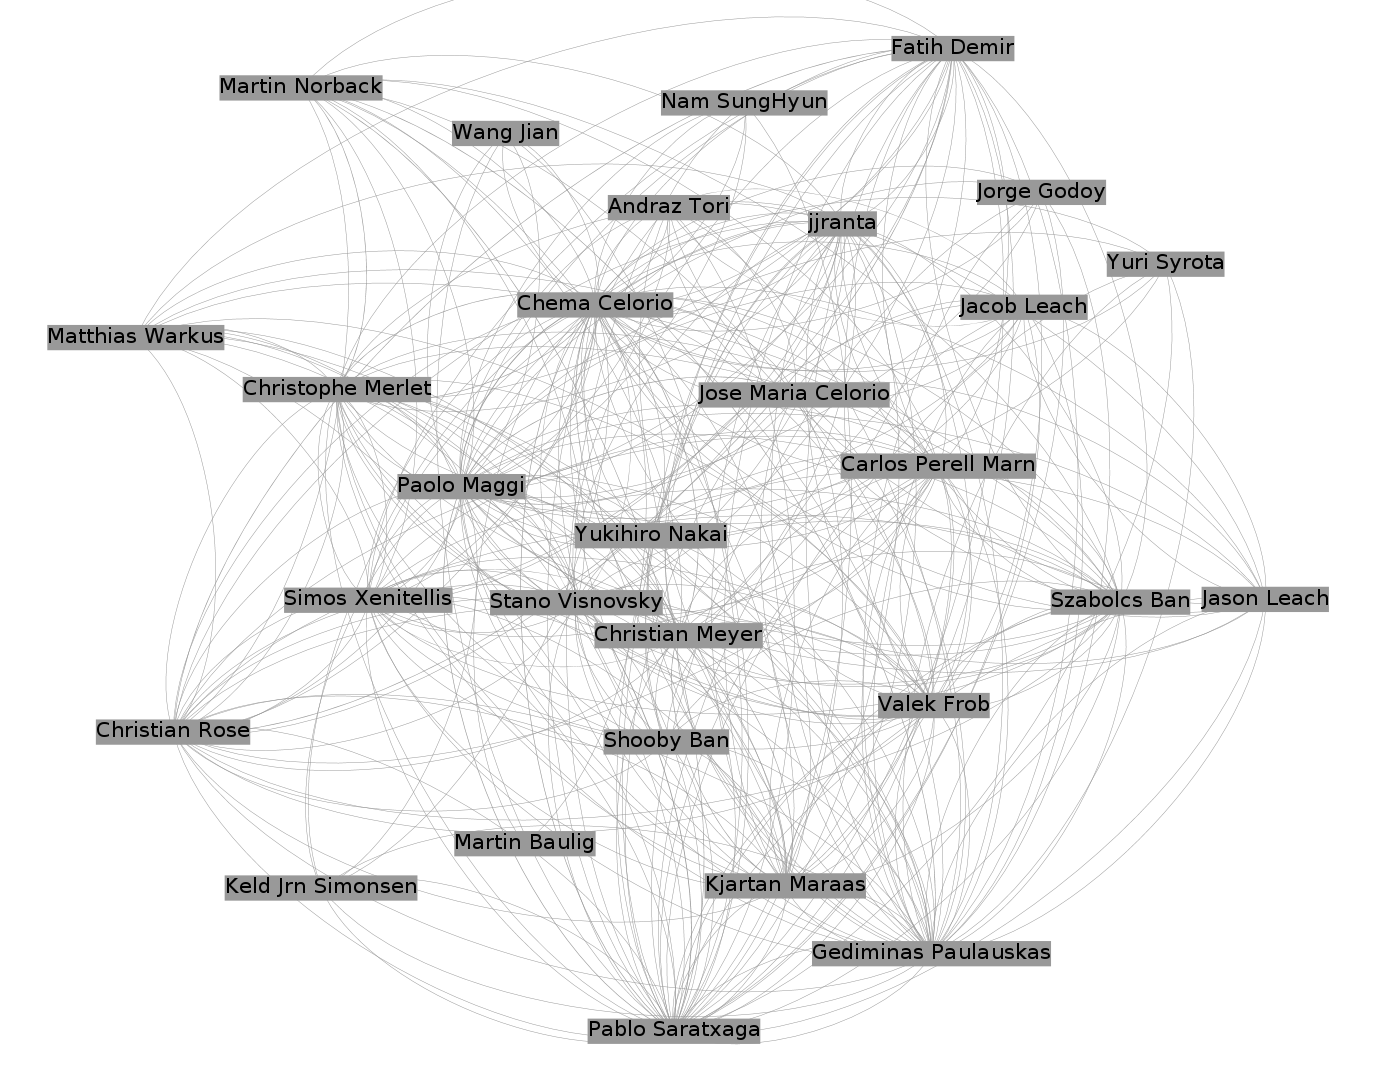
\includegraphics[scale=0.17]{g2001files.png} 
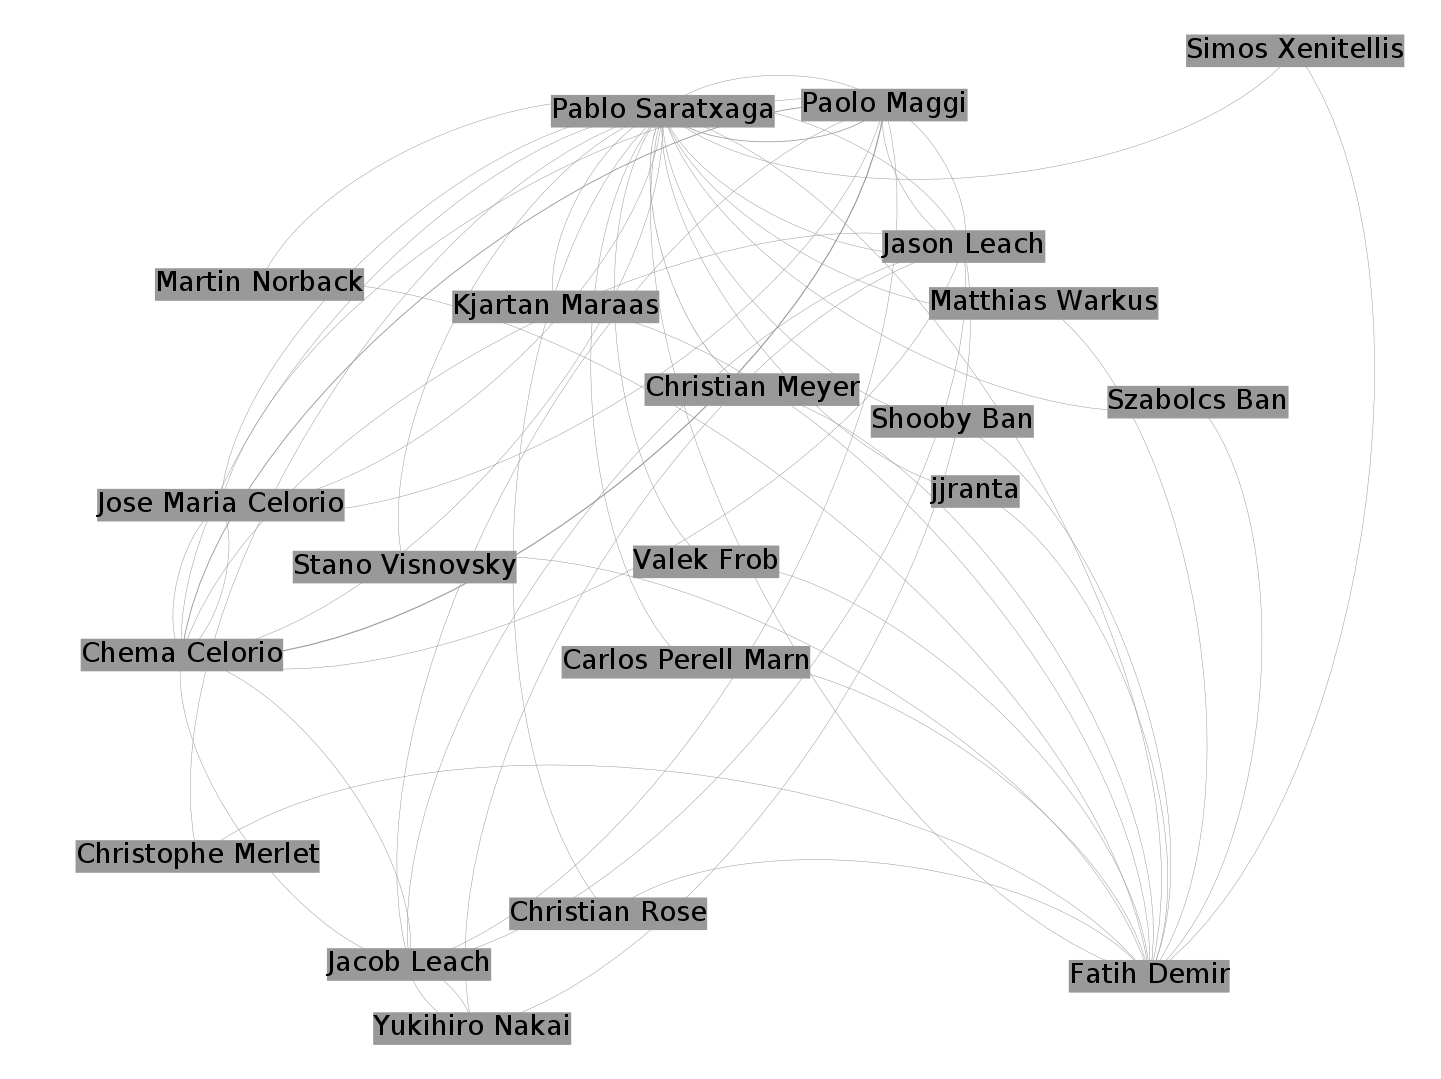
\includegraphics[scale=0.17]{g2001methods.png}
\caption{In-file (left) and In-method (right) collaboration graphs - 2001}
\label{fig:fixme1}
\end{center}
\end{figure}

Figure 2 shows the different graphs (In-file and In-method data) from
second-half of 2014.

\begin{figure}[ht]
\begin{center}
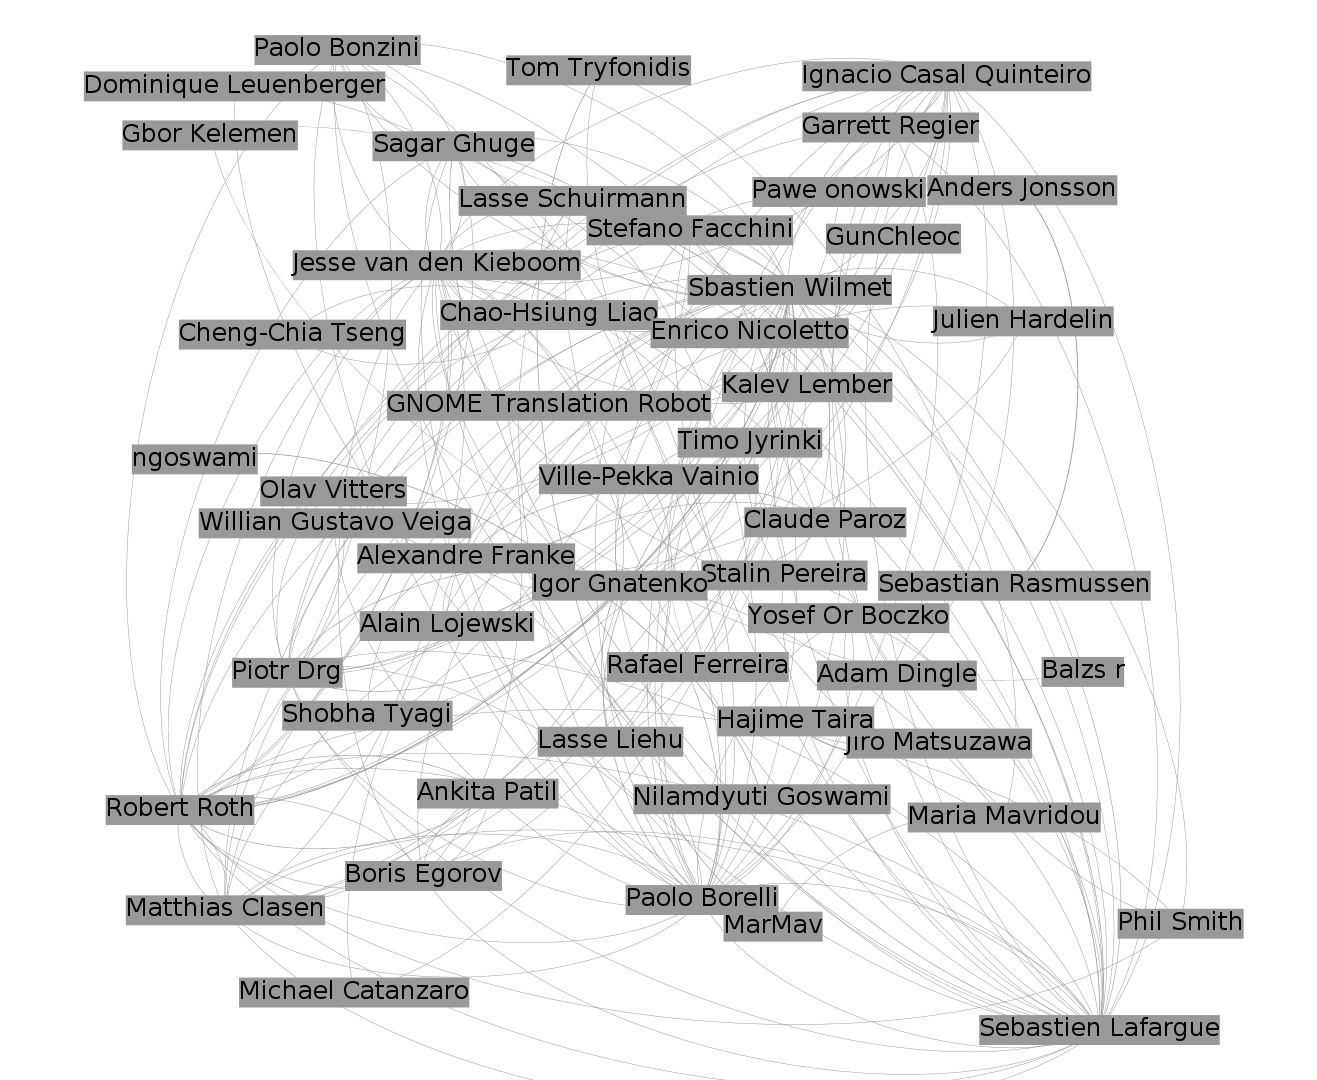
\includegraphics[scale=0.17]{g2014files.png} 
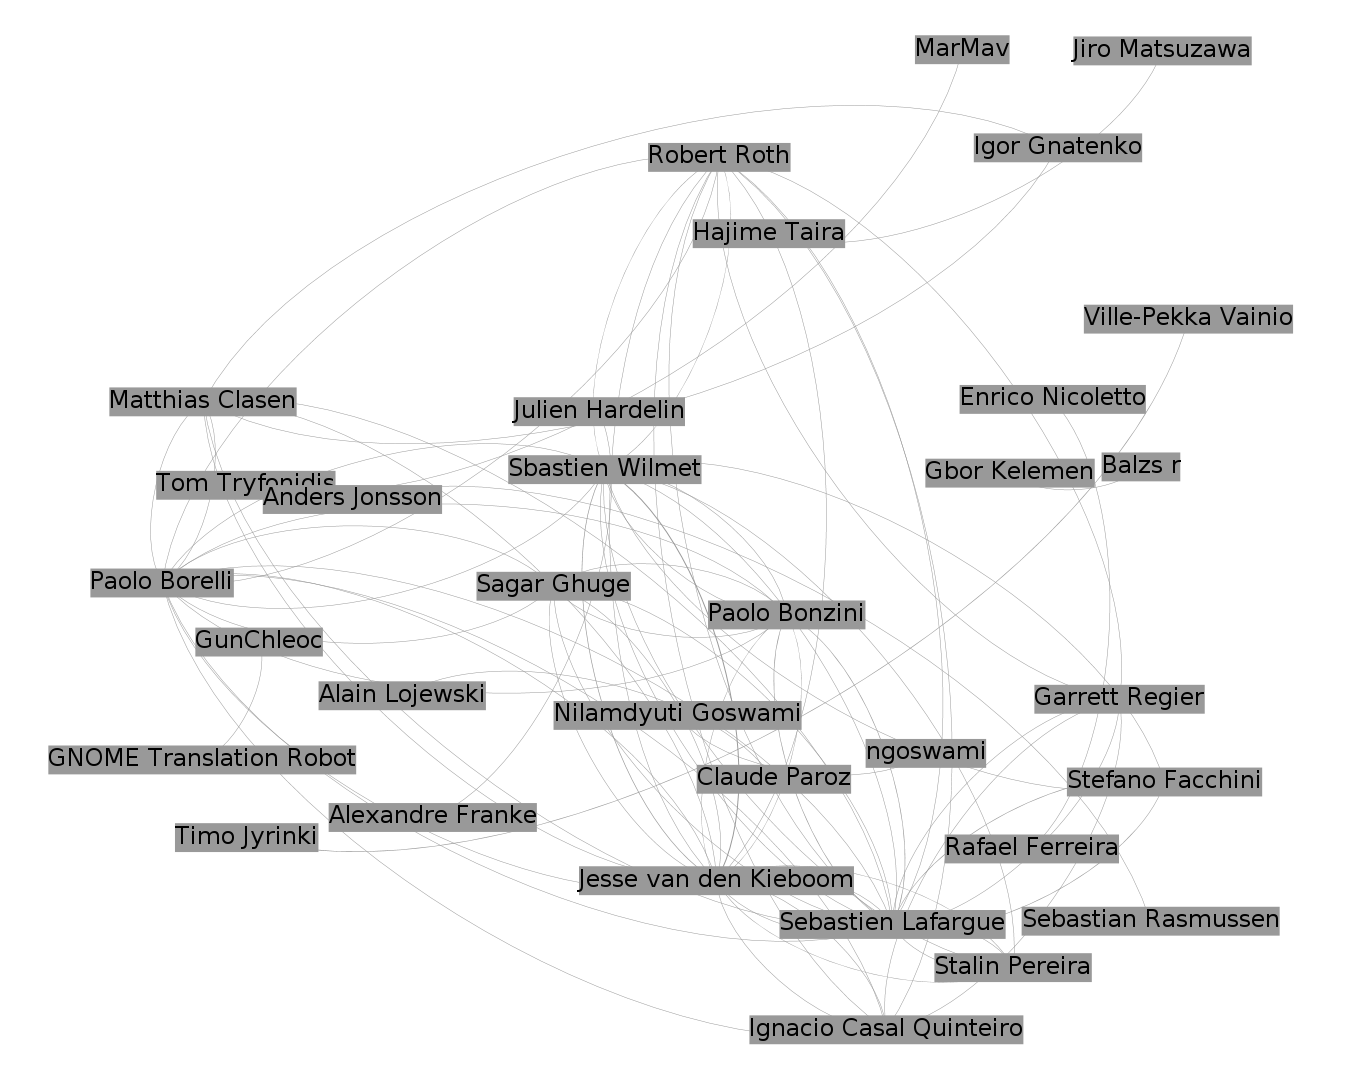
\includegraphics[scale=0.17]{g2014methods.png}
\caption{In-file (left) and In-method (right) collaboration graphs - 2014}
\label{fig:fixme2}
\end{center}
\end{figure}



\subsubsection{Tables}

All tables must be centred, neat, clean and legible. Do not use pencil
or hand-drawn tables. Table number and title always appear before the
table.

One line space before the table title, one line space after the table
title and one line space after the table. The table title must be
initial caps and each table numbered consecutively.

\begin{table}[ht]
\begin{center}
\caption{Sample Table}

\bigskip

\begin{tabular}{|l|l|r|}
\hline
A & B & 1\\ \hline
C & D & 2\\
E & F & 3\\ \hline
\end{tabular}
\end{center}
\end{table}


\subsubsection{Acknowledgements}

FIXME

\bibliographystyle{alpha} 
\bibliography{bib}
%inline the .bbl file directly for mailing to authors.

%\begin{thebibliography}{Com79}
%
%\bibitem[Com79]{Comer-btree}
%D.~Comer.
%\newblock The ubiquitous b-tree.
%\newblock {\em Computing Surveys}, 11(2):121--137, June 1979.
%
%\bibitem[Knu73]{Knuth-vol3}
%D.~E. Knuth.
%\newblock {\em The Art of Computer Programming -- Volume 3 / Sorting and
%  Searching}.
%\newblock Addison-Wesley, 1973.
%
%\end{thebibliography}

\end{document}


